\chapter{Methodology}\label{ch:methodology}

The next step for this senior project was to conduct an empirical study. Participants in this study have been selected among students who have had the class of Computer Science 112 or more advanced classes at Allegheny College. These students will in this paper be referred to as participants. 

Conducting the empirical study help me to determine how effective and useful the tools are. The results will tell me if participants were able to use the tools to assist them in finding logic based bugs in their code or if they were better off reading and analyzing the source code line by line to find the bugs.  
 
Ideally, the sample size should be at least 20 participants in this study. However, for practical reasons it has only been possible for me to get six students to participate and respond to my study. Therefore the results from my study cannot form the basis for a strong conclusion but rather give indications of the usefulness of the tools.  

I have developed four Java programs and each program has a bug in its code. These four programs are used in this study. All participants  used each of the three tools FindBugs, PMD, and Checkstyle to see if the tools could assist them in finding the bug in each of the four Java programs. In order to get the broadest feed back for the tools, it is essential that each participant get the chance to use each of the tools at least once. A participant may have to use one of the tools consecutively, but as long as each participant has used each of the tools at the end of the study, then the study has been properly completed. I have ensured that each participant used each of the tools at least once. 
 
There were preparations I needed to make for the empirical study to be conducted smoothly. Participants used the Eclipse Integrated Development Environment (Eclipse IDE) for the study. The Eclipse IDE that was provided to the participants had already the three tools FindBugs, PMD and Checkstyle installed. The rule sets in the tools are highly configurable and I had configured the rule sets to the default settings in all three tools - ready for the participants to use. 

I also provided instructions to participants on how to use the tools.  

In order to successfully perform this empirical study, I needed to get the approval of the Institutional Review Board (IRB). I was successful in getting the approval for my study. 

\begin{figure}[h]
	\begin{center}
		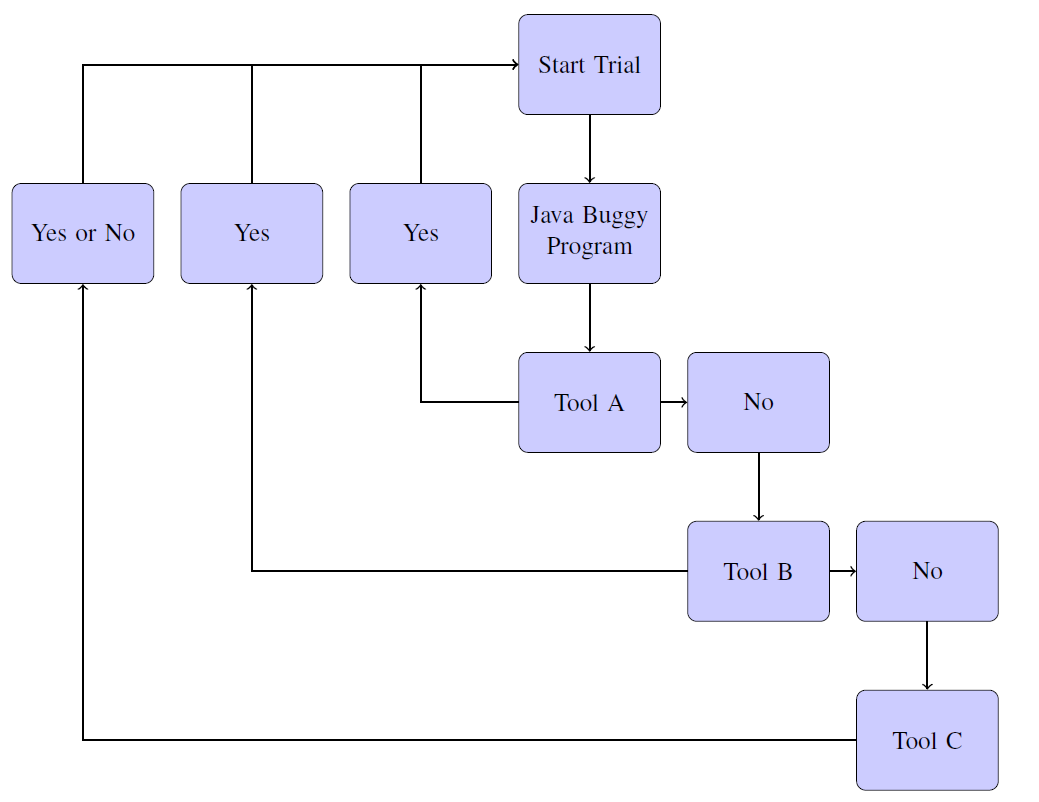
\includegraphics[width=1.15\textwidth]{Methodology.png}
	\end{center}
	\caption{The process of how this empirical study was conducted.}
	\label{fig:metholody}
\end{figure}

Figure 6.1 below displays how each buggy Java program was analyzed. In this study each participant was provided with one of the four buggy Java programs. The order of the Java programs in which the participants performed the analysis was determined by me to prevent any learning effect - meaning that the participants got experience and got better using the tools as they worked through this study. Then the participants were provided with one of the three tools FindBugs, PMD or Checkstyle  - again the tool was determined by me. After the participant had used the first tool to analyze the source code, there were two possibly outcomes. The tool could either have assisted the participant in finding the bug or the bug was not found. If the tool assisted in locating the bug, then the analysis of that Java program was completed and the participant continued by moving on to analyze the next buggy Java program. If the tool was not able to assist the programmer to locate the bug, I determined the next tool for the participant to use. If the second tool was successful in assisting locating the bug, the participant had completed analyzing the program and if not the third tool was provided to the participant. 

This process was repeated for each of the four buggy programs. Each participant had one hour to complete their tasks of analyzing the four programs. 

After the participants had completed the study, a survey was given to them. The survey asked the participants to answer the six questions listed below for each program:
\begin{itemize}
	\item Did you find the bugs?
	\item If yes, did FindBugs assist you in finding these bugs?
	\item If yes, did PMD assist you in finding these bugs?
	\item If yes, did Checkstyle assist you in finding these bugs
	\item Would you use any of these tools in the future for finding logic based bugs?
	\item Suggestion to further improve these tools.
\end{itemize}

The responses from the survey told me results from the study and were used to draw the conclusion.   

I have developed four Java programs each with a bug in its code. The four programs are intended to represent some of the most common mistakes made by Java programmers. I have chosen the bugs based on informal conversations with common students and professors and by searching the Internet. 

The first Java program that was used in this study should convert the numbers ranging from -5 to 32 into the binary representation. The program has a 'for loop' that contains an iteration of the numbers from -5 to 32. However, when participants ran the program, they learned that the program would output the binary representation of the number 33. It is because there is a bug with the 'for loop' in the code. Having a semi-colon right before the program block, will cause the 'for loop' to continue to iterate through the loop without going to the code inside the block. The semicolon was misplaced, as it should not be there at all.

The second Java program calculated the velocity and velocity squared by getting the kinetic and mass as input. As long as mass is not equal to zero the program should run properly, since division with zero is not possible. The program will print out 4 lines. The first and second line will display the kinetic and mass given as input. The third line will display the calculated velocity squared and the last line will display the calculated velocity. The output for velocity squared is incorrect because the equation used in the calculation is incorrect. In the source code the equation is as follows
\begin{lstlisting}
velocity_squared = 3 * (kinetic / mass);
\end{lstlisting}
This equation is incorrect. The equation in the Java source code to calculate velocity squared correctly should have been the following:
\begin{lstlisting}
velocity_squared = 2 * (kinetic / mass);
\end{lstlisting}
The bug in this program is the incorrect number used to calculate the velocity squared.
 
 
 The third Java program takes a text file as input. The file includes a list of airlines that are collaborating so miles can be transferred from airline to another. For example, miles can be  transferred from Air Canada to Ocean Air. However, that is not possible when running the program. The bug is in the canRedeem() method. In the very first 'if' statement, when two strings of current and goal are compared, the '==' operator is used. This is incorrect and the .equals() method should be used instead. The '==' operator checks whether the references to the objects are equal, and the .equals() method checks for the actual contents of the string.
 
 The last Java program was a program of the game  tic-tac-toe. The game was set to a difficult level so the only outcome of the game was either the computer was winning or the game ended in a tie. When the program ran, the output did not display correctly. The bug was in the printBoard() method. In the printBoard() method  a switch statement with 3 cases is used. Both Case 0 and Case 1 need a break statement. However, as can be seen in the source code, there is only a break statement after case 1.